\documentclass[11pt]{article}
\usepackage{setspace}
\setstretch{1}
\usepackage{amsmath,amssymb, amsthm}
\usepackage{graphicx}
\usepackage{bm}
\usepackage[hang, flushmargin]{footmisc}
\usepackage[colorlinks=true]{hyperref}
\usepackage[nameinlink]{cleveref}
\usepackage{footnotebackref}
\usepackage{url}
\usepackage{listings}
\usepackage[most]{tcolorbox}
\usepackage{inconsolata}
\usepackage[papersize={8.5in,11in}, margin=1in]{geometry}
\usepackage{float}
\usepackage{caption}
\usepackage{esint}
\usepackage{url}
\usepackage{enumitem}
\usepackage{subfig}
\usepackage{wasysym}
\newcommand{\ilc}{\texttt}
\usepackage{etoolbox}
\usepackage{algorithm}
\usepackage{changepage}
% \usepackage{algorithmic}
\usepackage[noend]{algpseudocode}
\usepackage{tikz}
\usetikzlibrary{matrix,positioning,arrows.meta,arrows}
\patchcmd{\thebibliography}{\section*{\refname}}{}{}{}
% \PassOptionsToPackage{hyphens}{url}\usepackage{hyperref}

\providecommand{\myceil}[1]{\left \lceil #1 \right \rceil }
\providecommand{\myfloor}[1]{\left \lfloor #1 \right \rfloor }


\begin{document}



\title{\textbf{CSDS 455: Homework 20}}

\author{Shaochen (Henry) ZHONG, \ilc{sxz517}}
\date{Due and submitted on 11/02/2020 \\ Fall 2020, Dr. Connamacher}
\maketitle

\textit{I have consulted Yige Sun and Yuhui Zhang for the following problems.}

\section*{Problem 1}

\textit{I have consulted and cited visual aids from \url{https://cseweb.ucsd.edu/classes/sp11/cse202-a/lecture7-final.pdf}.}

Let \ilc{I(u)} to be the maximum independent set of the subtree rooted to node \ilc{u}. We will have two cases:


\begin{figure}[H]
    \centering
    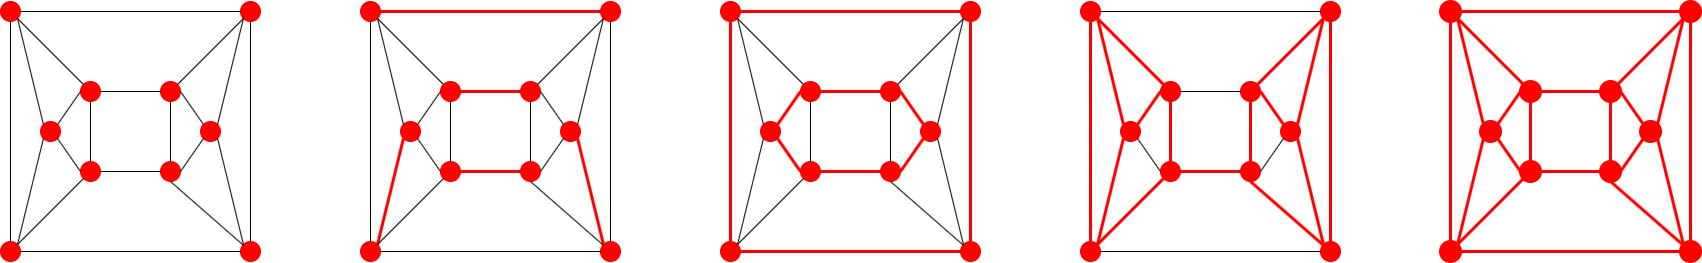
\includegraphics[width=0.4\linewidth]{{fig/fig_p1.png}}
\end{figure}

\begin{itemize}
    \item \ilc{I(u)} includes \ilc{u}.
    \item \ilc{I(u)} does not \ilc{u}, but includes children of \ilc{u}.
\end{itemize}


\noindent Since the goal is to maximize the size of the set, we have \ilc{I(u)} to be:

\begin{equation*}
    I(u) = \max \{\sum_{\text{child $v$ of $u$}} I(v), \ \  1 + \sum_{\text{grandchild $w$ of $u$}} I(w)\}
\end{equation*}

Then we may simply do a postorder traversal from leaves to the root of the tree, the runtime will therefore be $O(|T|)$.

\section*{Problem 2}

We may use the same algorithm proposed in \textit{Problem 1}. A leave 

\section*{Problem 3}



\end{document}